%!TEX root = ../main.tex
\chapter{MARCO TEÓRICO}
\label{ch2:MarcoTeorico}

\section{Acrónimos}
En el archivo auxiliar ``Aux\_files/Glossary.tex'' se definen los términos del glosario.
Es útil usar acrónimos: \gls{ITAM}. Si se usa por segunda vez ya no se expande: \gls{ITAM}. 

\section{Glosario}
Para usar un término del glosario: \gls{Wi-Fi}.

\section{Citas}
En el archivo auxiliar ``Aux\_files/FuentesConsultadas.bib'' se define la bibliografía. Se puede usar como: \cite{turing2009computing}.


\section{Imágenes}
Importar imágenes (con citas):

\label{robocup-ssl}
\begin{figure}
	\centering
		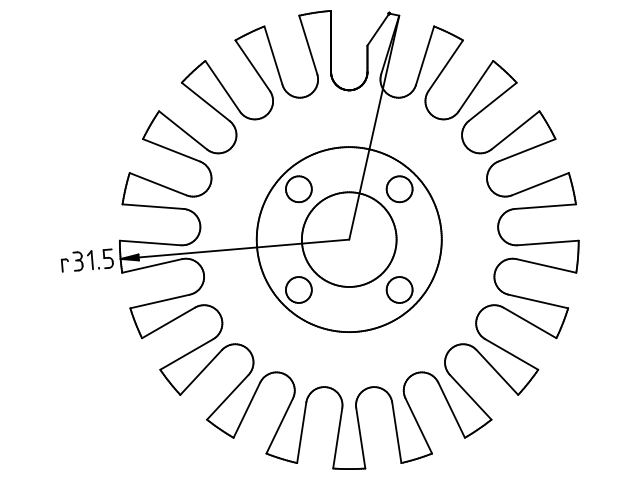
\includegraphics[width=.8\textwidth,height=.8\textheight]{rueda.png}
	\caption{Rueda Omnidireccional \protect\cite{itam-gary} }
	\label{fig:SP}
\end{figure}

Se pueden usar imágenes eps y ponerlas en página completa giradas.
\begin{sidewaysfigure}
	\centering
		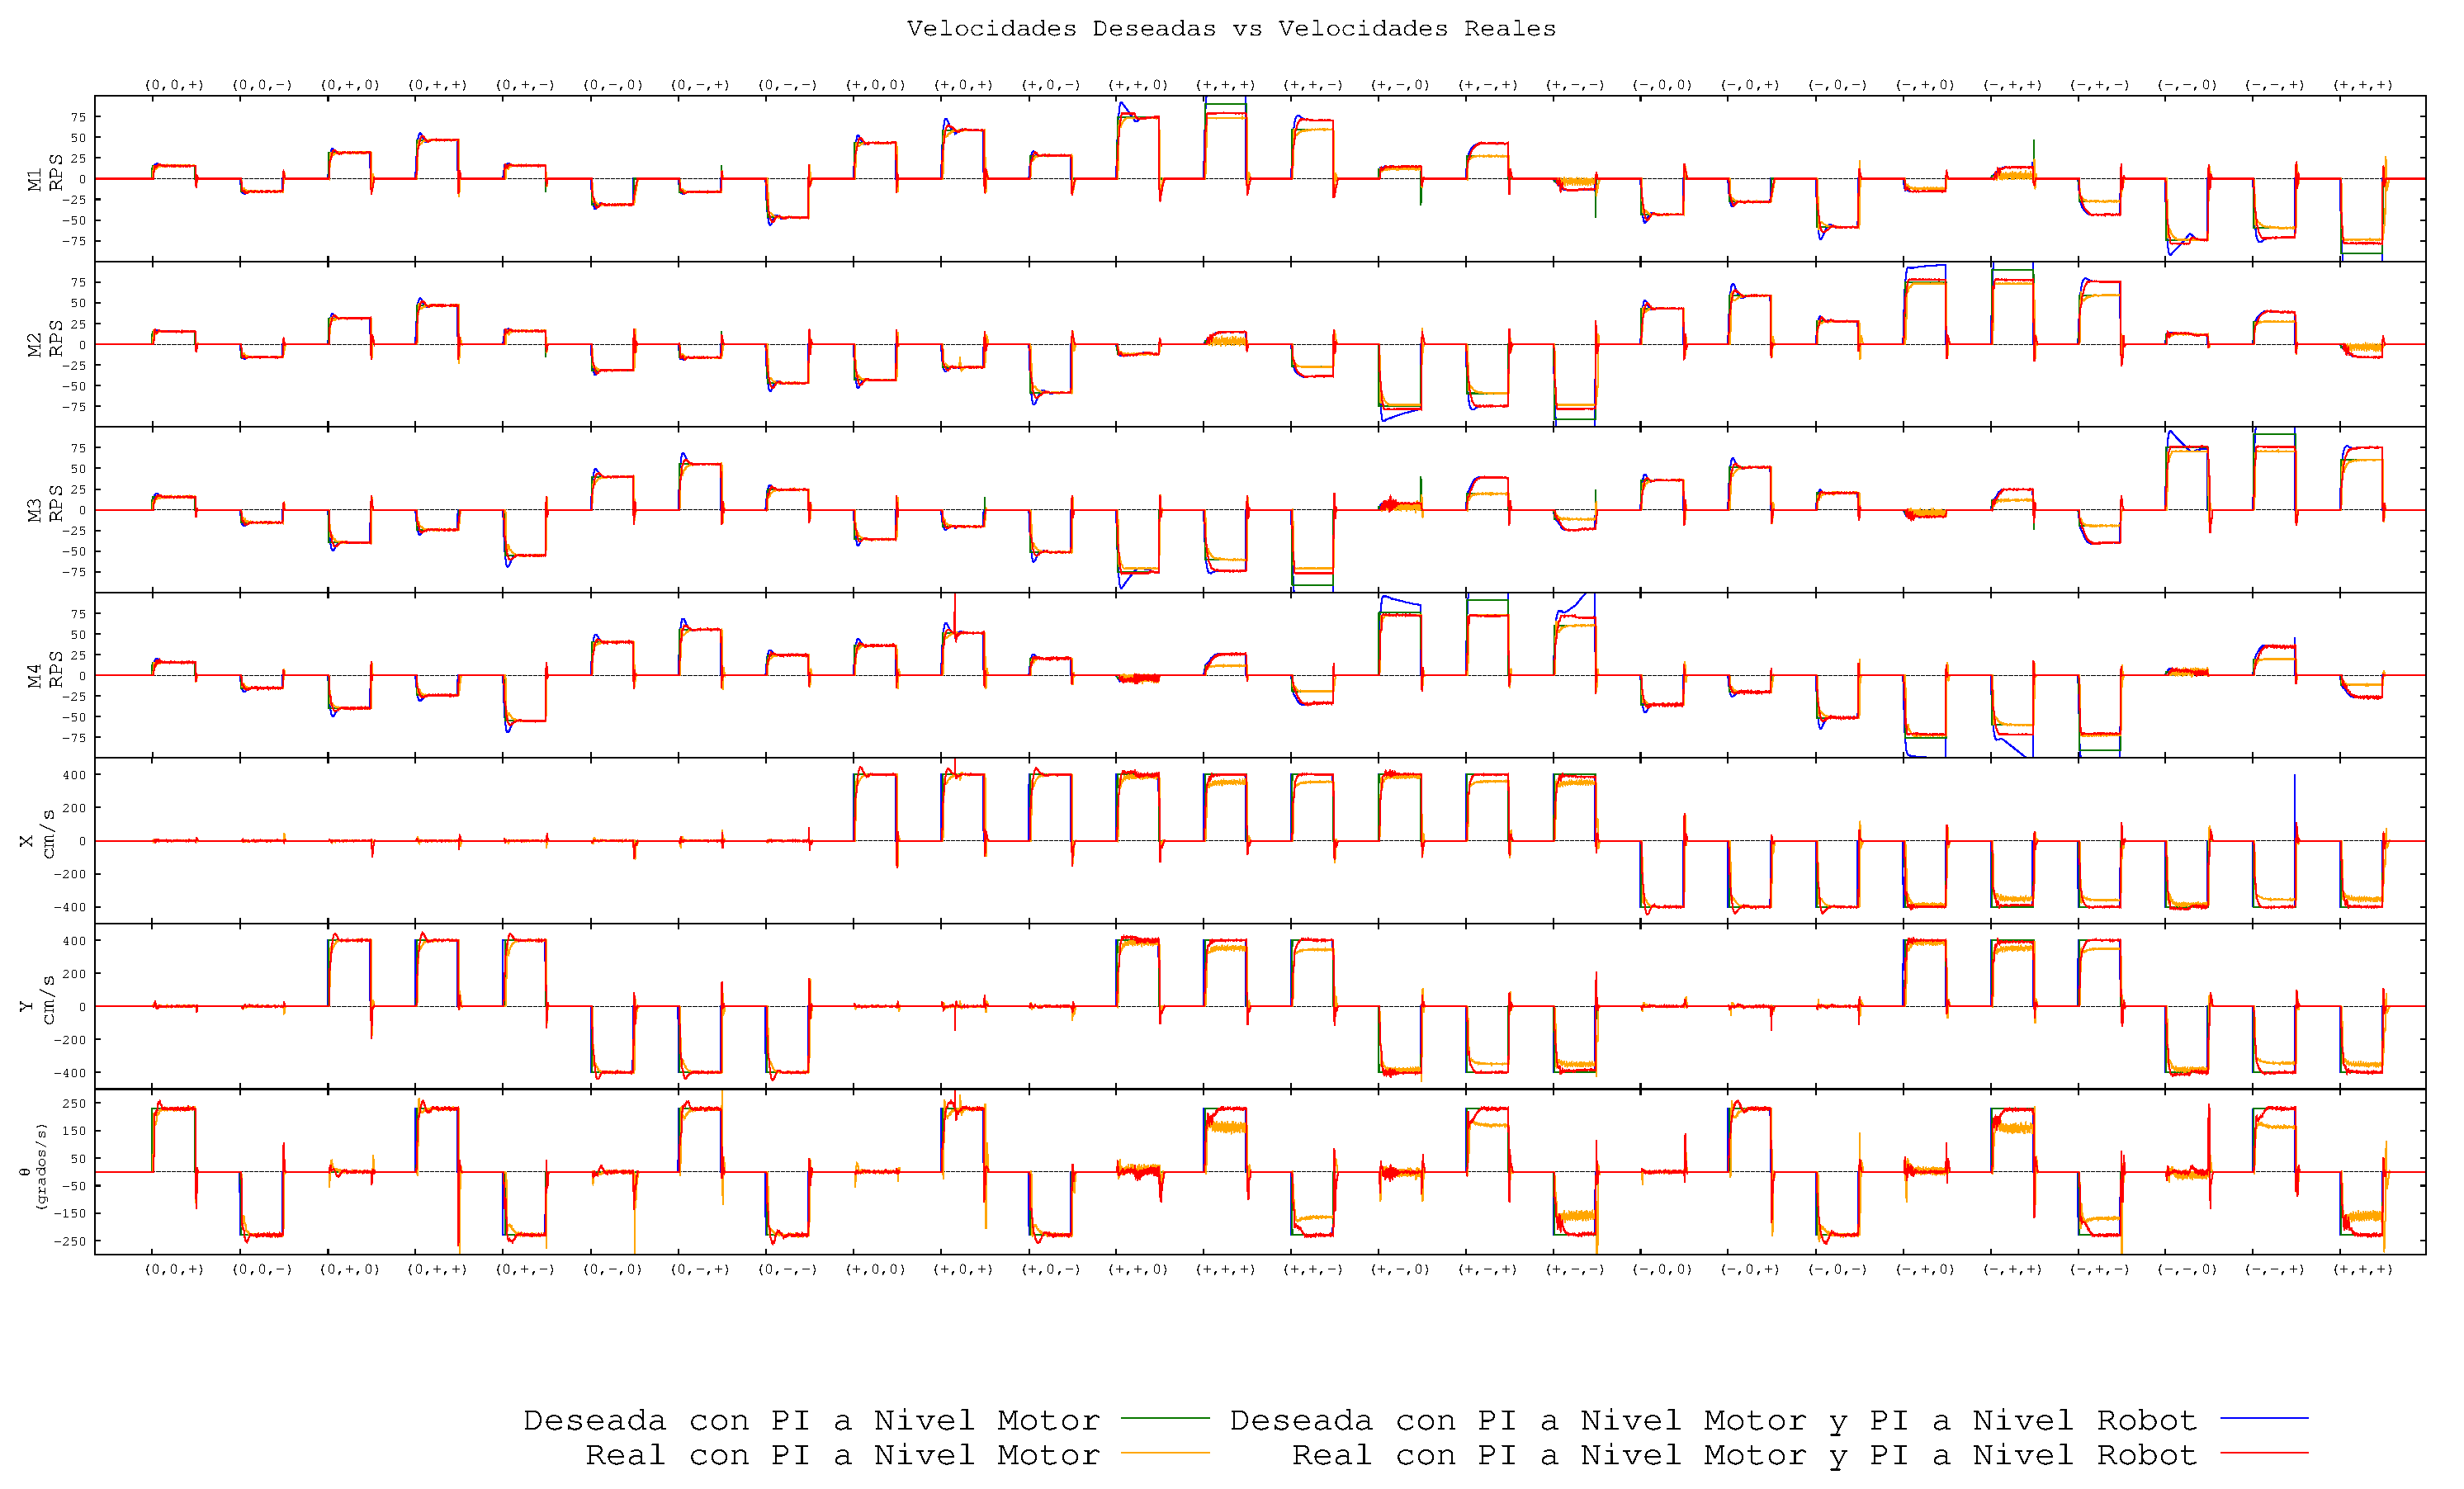
\includegraphics[width=\textwidth,height=0.9\textheight]{Figures/160517-vels-motVSmotrob_slide.eps}
	\caption{Velocidades Deseadas vs Velocidades Reales}
	\label{fig:vels_real_vs_des_mot}
\end{sidewaysfigure}

% \label{robocup-ssl}
% \begin{figure}
% 	\centering
% 		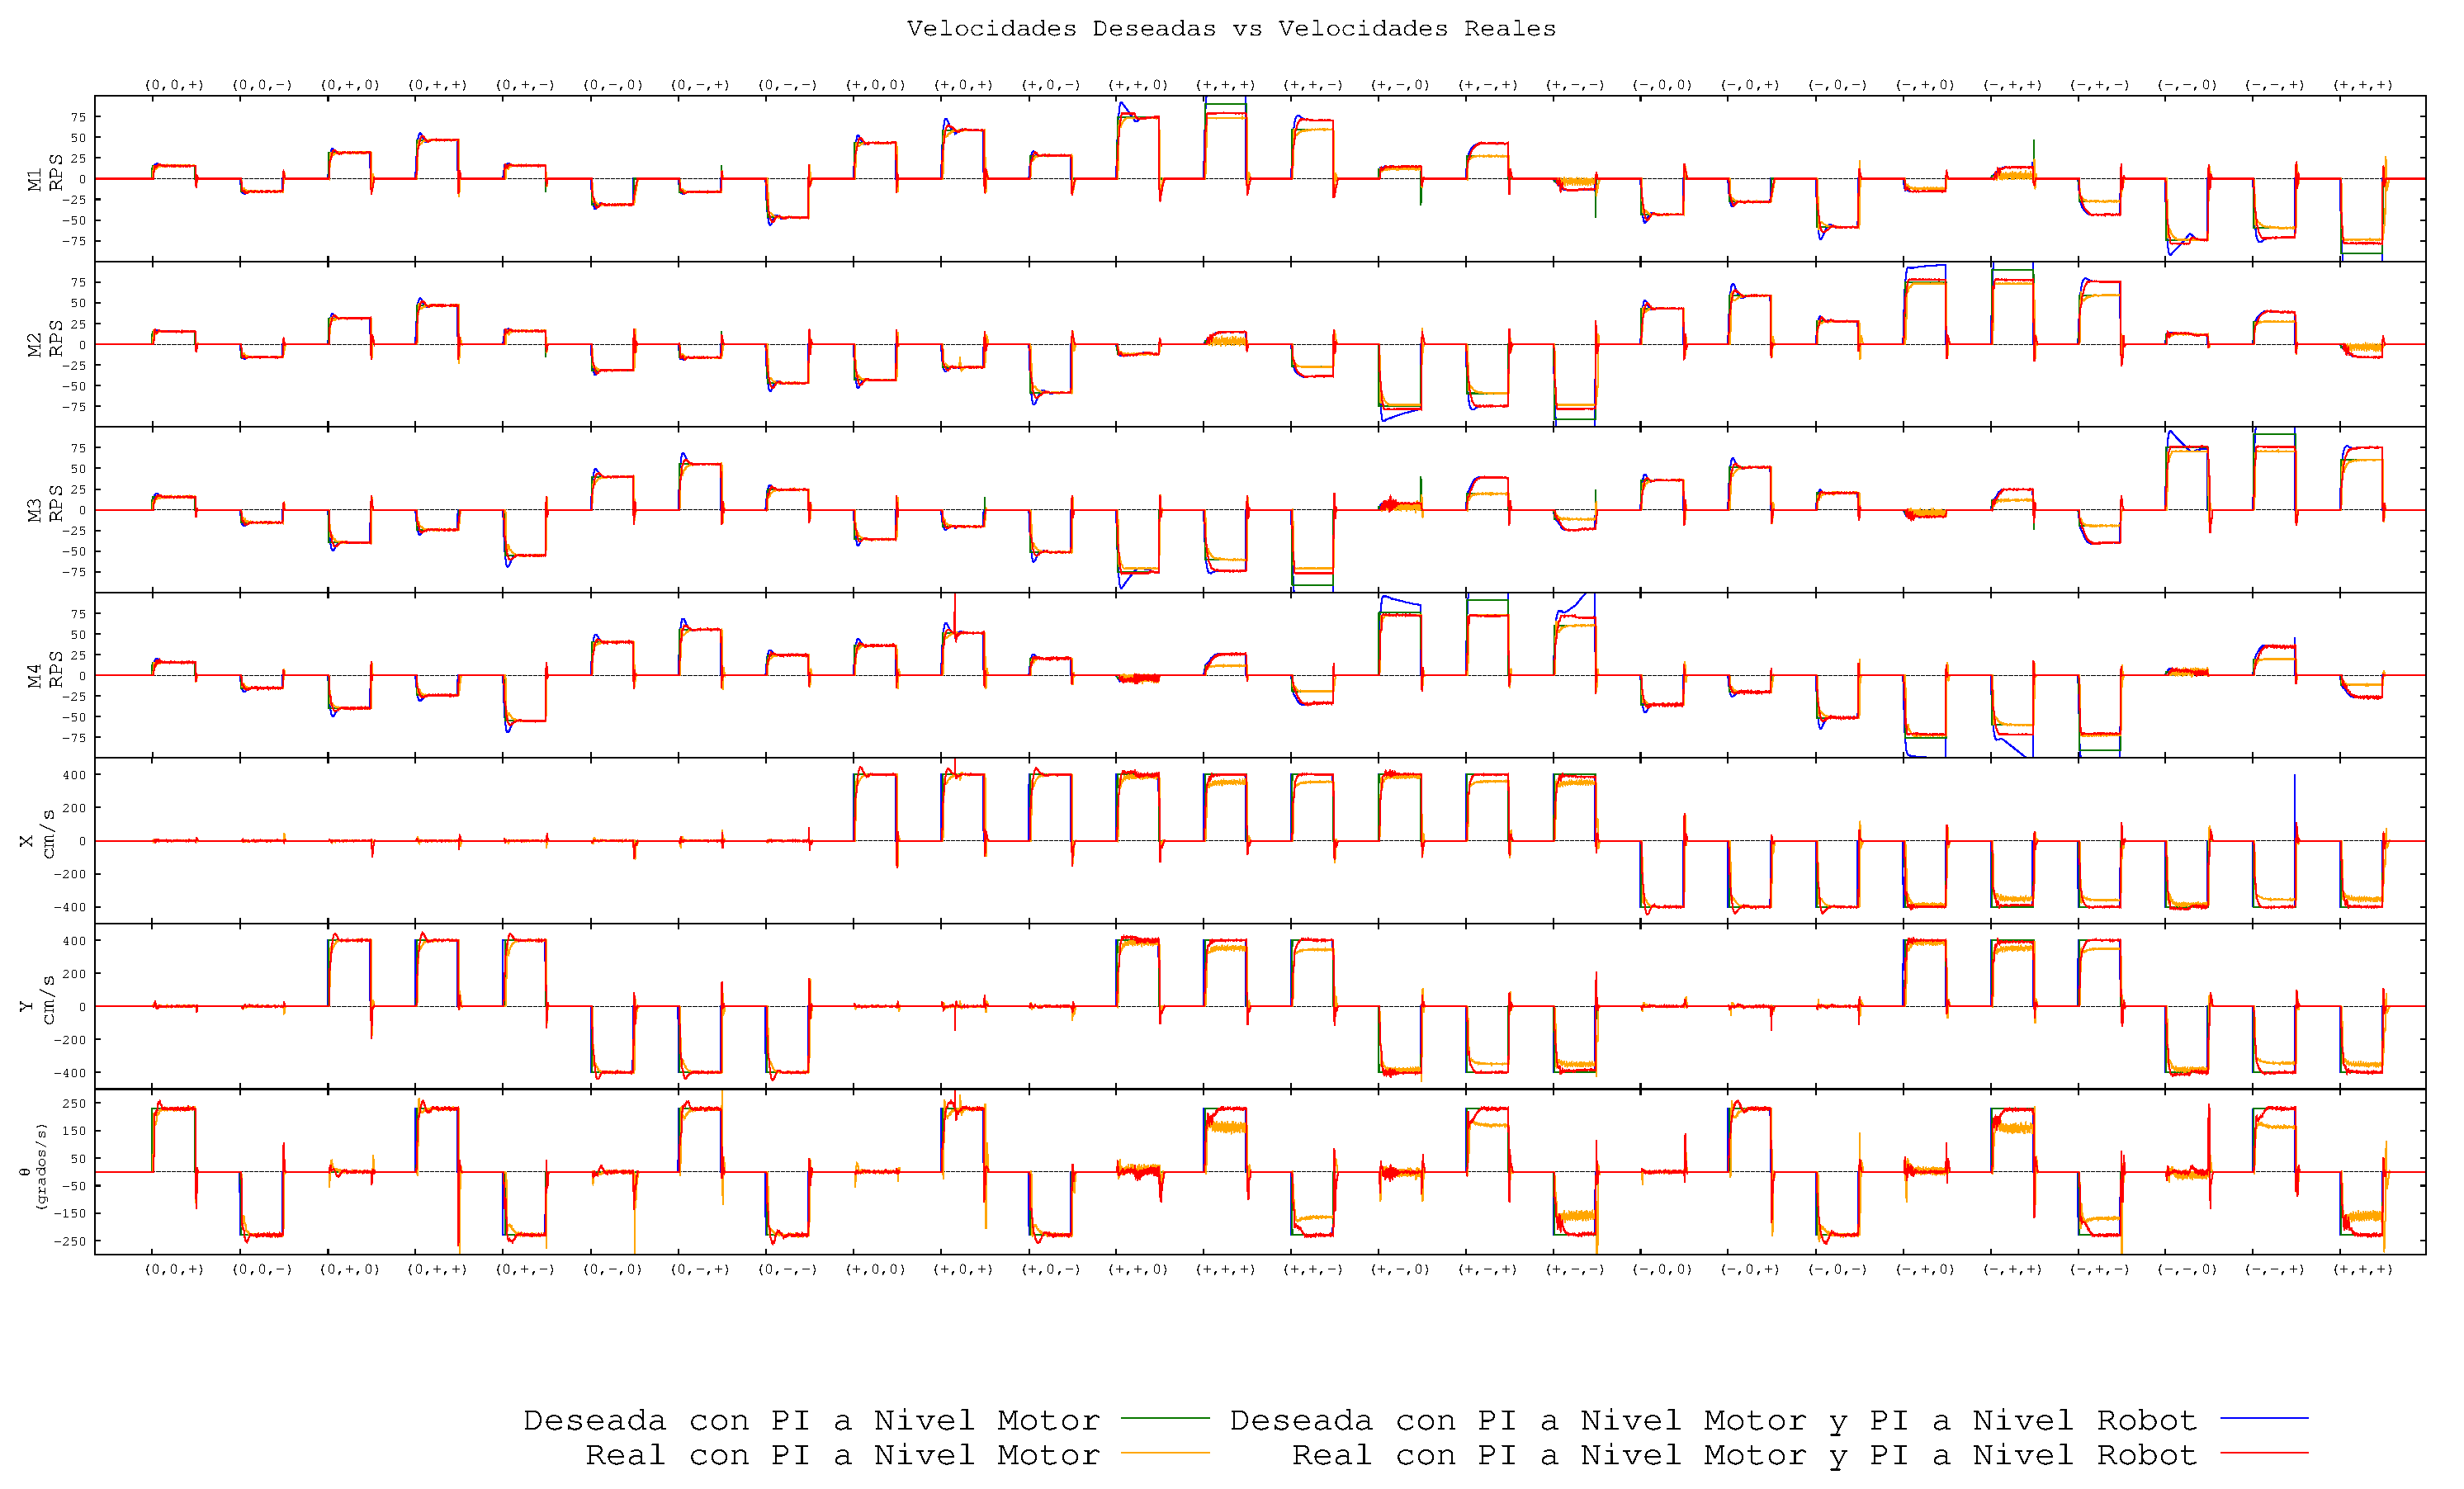
\includegraphics[width=8cm]{Figures/160517-vels-motVSmotrob_slide}
% 	\caption{Rueda Omnidireccional}
% 	\label{fig:SP}
% \end{figure}


% Una categoría de RoboCup, la \gls{SSL} se enfoca enfoca en la cooperación inteligente de agentes además del control en un ambiente altamente dinámico con un sistema híbrido centralizado-distribuido. Un juego de \gls{SSL} de RoboCup, consiste en dos equipos de seis robots cada uno que tienen acceso a un sistema de visión global así como un árbitro. Cada robot debe cumplir con las características especificadas en las reglas F180, entre las cuales se encuentran:
% \begin{itemize}
% \item No puede tener objetos que sean peligrosos para otros robots o para humanos.
% \item Debe caber dentro de un cilindro de 180 mm de diámetro y 150 mm de alto.
% \item El área superior debe cumplir con el \gls{SP} (Fig. \ref{fig:SP}).
% \item El área externa debe ser obscura y con acabado mate.
% \item No debe dañar la cancha al moverse.
% \item Puede utilizar comunicación inalámbrica con computadoras fuera de la cancha.
% \item Debe ser completamente autónomo durante el partido.
% \end{itemize} \par

% \begin{figure}
% 	\centering
% 		\includegraphics[width=8cm]{Ssl_dataflow.png}
% 	\caption{Arquitecura de un equipo SSL. \protect\cite{sslWiki} }
% 	\label{fig:Ssl_dataflow}
% \end{figure}

% Como se muestra en la Fig. \ref{fig:Ssl_dataflow}, un equipo de RoboCup \gls{SSL} está conformado por al menos seis robots móviles y una computadora. La computadora debe poder conectarse y procesar la información proporcionada por los sistemas globales de \gls{SSL}. Igualmente, determinar las estrategias necesarias y comunicarlas a los robots. 

% Los jugadores en \gls{SSL} son robots omnidireccionales como jugadores de fútbol. 
% La pose de los robots se obtiene con un sistema de visión integrado por cámaras en la parte superior de la cancha además del software provisto por la liga para el procesamiento de imágenes que detecta el \gls{SP} de cada robot. 

% Varios equipos se han destacado a lo largo de la historia de la competencia.
% \textit{Cornell Big Red} fue uno de los primeros ganadores de la liga, explorando diversos tipos de ruedas omnidireccionales como la ortogonal \cite{d2000cornell} y posteriormente ruedas universales \cite{purwin2003cornell} con un control basado en torque para evitar sobre calentamiento en las escobillas de los motores y un segundo lazo para la orientación del robot utilizando un giroscopio. \textit{FU-Fighters} fue uno de los primeros en utilizar ruedas con rodillos perpendiculares \cite{egorova2003fu}. \textit{Skuba} también ha utilizado control PI basado en torque, con motores sin escobillas \cite{chaisoskuba}. 

% Debido al tamaño de los robots, el consumo de energía es una de las características más importantes de los robots. Por esto, se han explorado diversas opciones de cómputo a bordo del robot. Por ejemplo, los equipos del \gls{ITAM} utilizaban \gls{DSP} \cite{itam-torres-ssl} mientras \textit{TIGERS Mannheim}, utiliza un microcontrolador \cite{rylltigers}. Otra opción popular es una FPGA como la usada por \textit{MRL} \cite{poudeh2016mrl}. \textit{ZJUNlict}, en cambio, usa una FPGA donde implementan un microcontrolador \cite{zhao2013zjunlict}. Por último, equipos como \textit{Skuba} utilizan tanto una \gls{FPGA} como un microcontrolador.


% El equipo Eagle Knights del \gls{ITAM} ha participado en la RoboCup \gls{SSL} desde 2006 en cinco ocasiones.

% Como consecuencia de la obsolescencia de la implementación anterior además de diversos problemas con la misma, se determinó la necesidad de realizar una nueva implementación para poder competir de manera satisfactoria en futuras RoboCups. Es necesario la incorporación de tecnologías que antes no eran accesibles ya fuera por costo o por ser de gran tamaño respecto al robot.

% Algunos de los trabajos realizados en el \gls{ITAM} relacionados con RoboCup \gls{SSL} incluyen \cite{itam-torres-ssl} donde se muestra una implementación de un sistema de inteligencia para controlar robots de \gls{SSL}. En \cite{misael-itam-dribbler} se muestra el diseño del sistema para controlar la pelota de versiones anteriores del robot. Un control de trayectorias para los robots \gls{SSL} se detalla en \cite{r-raftrcssl-2009-itam}. 


% \section {Estándares y Códigos Relevantes}

% Se toman las reglas de la \gls{SSL} \cite{SSLrules2016} como el estándar que el robot debe cumplir. Durante el desarrollo se seleccionaron estándares y códigos específicos de acuerdo a la funcionalidad deseada.

% Los materiales utilizados para manufacturar las piezas propias son \gls{ABS} y \gls{HIPS}. Específicamente, se utilizan los productos de la marca \textit{Zortrax}: Z-ABS \cite{z-abs} y Z-HIPS \cite{z-hips}. Para ensamblar éstas piezas se utilizan tornillos M3x5 o M3x12. Adicionalmente, se utilizan tornillos 6-32 UNC para acoplar dos piezas comerciales debido a las características de éstas. Un tornillo $\frac{1}{4}^{\prime\prime} -20\times 2^{\prime\prime}$ como eje de cada rueda. Por último, se utilizan engranes de \textit{pitch} 32 con 20 grados de ángulo de presión. 

% Para la alimentación eléctrica, se utilizan baterías \textit{LiPo} 2S y 3S \cite{salt2012understanding}. Se utilizan componentes TTL para los circuitos propios. La tarjeta de desarrollo utilizada opera con LVTTL.

% Para la comunicación entre componentes se utiliza \gls{SPI} 0 \cite{davis2013serial}, \gls{UART} o \gls{PWM} \cite{valvano2012embedded}. Para la comunicación inalámbrica se utiliza XBee \cite{xbee_wifi_manual}, específicamente la implementación del protocolo IEEE 802.11n \cite{tanenbaum2003computer}; ésta comunicación se realiza mediante \gls{UDP} \cite{tanenbaum2003computer}.

% \section {Robot Móvil Omnidireccional}
% \label{sec:MovOmni}
% \begin{figure}
% 	\centering
% 		\includegraphics[width=4cm]{omni_rojas}
% 	\caption{Ejemplo de Rueda Omnidireccional \protect\cite{rojas2005short} }
% 	\label{fig:omni_wheel_gral}
% \end{figure}
% \EXCISE{
% Un robot omnidireccional (holonómico) se puede mover en un plano entre cualesquiera dos poses arbitrarias $A$ y $B$ trasladándose sobre una línea recta mientras gira sobre su propio eje \cite{rojas2005short}. Las poses $A$ y $B$ se caracterizan por una posición $(x,y)$ y una orientación $\theta$ con respecto a un sistema de referencia. Se depende de dos características para tener movimiento omnidireccional: rueda y base del robot. \par

% Se puede lograr movimiento omnidireccional con un robot de ruedas concéntricas que tenga al menos 3 ruedas omnidireccionales colocadas con distintos ángulos de separación \cite{rojas2006holonomic}. Ruedas adicionales proporcionan redundancia que permite cierta tolerancia a fallas por lo que el robot de 4 ruedas es muy popular. \par
% }


% Un robot móvil omnidireccional se puede mover en un plano entre cualesquiera dos poses arbitrarias $A$ y $B$ trasladándose sobre una línea recta mientras gira sobre su propio eje \cite{rojas2005short}. Las poses $A$ y $B$ se caracterizan por una posición $(x,y)$ y una orientación $\theta$ con respecto a un sistema de referencia. Se puede lograr movimiento omnidireccional con al menos 3 ruedas omnidireccionales concéntricas colocadas con distintos ángulos de separación \cite{rojas2006holonomic}. Ruedas adicionales proporcionan redundancia que permite cierta tolerancia a fallas por lo que el robot de 4 ruedas es muy popular.

% La principal ventaja de los robots omnidireccionales es su maniobrabilidad.

% El OmniBot de la NASA fue desarrollado como un robot altamente maniobrable para ambientes peligrosos \cite{houshangi1999omnibot}. El Airtrax ATX-3000 es un levantacargas para trabajo en almacenes \cite{aduascualictei2011practical}. El \textit{OMNI-chair} es una silla de ruedas omnidireccional diseñada para darle mayor capacidad de movimiento a su usuario \cite{borgolte1998architectural}.

% Existen diversos diseños de rueda omnidireccional, dos tipos son ortogonales y universales \cite{ashmore2002omni}. Las ruedas ortogonales consisten en dos esferas cortadas por dos planos paralelos; el eje de la rueda es perpendicular a las superficies recortadas. Las ruedas universales consisten en una rueda con rodillos en un ángulo en la periferia, un diseño muy popular es la rueda Mecanum, Fig. \ref{fig:kuka_omni}. Sus principales limitaciones son el diseño complejo (conceptual y físico) así como el gran espacio que ocupan los rodillos. Otro diseño popular de rueda universal por su diseño compacto cuenta con rodillos alineados al eje principal de la rueda. 

% También existen las ruedas orientables (Fig. \ref{fig:orient_wheel}) que necesitan de un motor extra por rueda para orientar la rueda al ángulo deseado. La rueda HOG (Cardán semiesferica omnidireccional por sus siglas en inglés) es una superficie giratoria semiesférica la cual se encuentra montada en una suspensión Cardán. Esta rueda se mueve por motores, de manera inversa al mecanismo de un \textit{mouse} mecánico.

% \EXCISE{
% La base del robot determina tanto el número de ruedas que se utilizarán así como la posición de las ruedas. La rueda debe ser omnidireccional existiendo varios diseños. La más común se basa en tener en toda la circunferencia rodillos pasivos con sentido de giro en ángulo de 90º respecto al sentido de giro de la rueda, como se muestra en la Fig. \ref{fig:omni_wheel_gral}. Otro tipo de rueda omnidireccional se conoce como \textit{Mecanum} o \textit{Rueda Sueca}, siendo una variación de la primera al tener los rodillos en cierto ángulo distinto de 90º, generalmente 45º. También existen las ruedas orientables (Fig. \ref{fig:orient_wheel}) que necesitan de un motor extra por rueda para orientar la rueda al ángulo deseado. Otro diseño se conoce como rueda HOG (Cardán semiesferica omnidireccional por sus siglas en inglés) la cual consiste en una superficie giratoria semiesférica la cual se encuentra montada en una suspensión Cardán. El último diseño consiste en una esfera movida por motores, de manera inversa al mecanismo de un \textit{mouse} mecánico. \par
% }

% \begin{figure}
% 	\centering
% 		\includegraphics[width=4cm]{orientable_wheel}
% 	\caption{Ejemplo de Rueda Orientable \protect\cite{neobotix-orientable-wheel}}
% 	\label{fig:orient_wheel}
% \end{figure}

% \begin{figure}
% 	\centering
% 		\includegraphics[width=6cm]{kuka_omni_robot}
% 	\caption{Kuka Omnidirectional Robot \protect\cite{bischoff2011kuka}}
% 	\label{fig:kuka_omni}
% \end{figure}
% %%%%%%%%%%%%%%%%%%%%%%%%%%%%%%%%%%%%%%%%%%%%%%%%%%%%%%%%%%%%%%%%%%%%%%%%%%%%%%%%%%%%%

% \EXCISE{
% El robot presentado en este trabajo se probó inicialmente en el contexto de la \emph{Small Size League} de la RoboCup \cite{sslWiki}, o SSL, que utiliza robots omnidireccionales como jugadores de fútbol. Los robots deben caber en un cilindro de 18 cm de altura por 15 cm de diámetro y deben moverse sin dañar la carpeta que forma la cancha. La pose de los robots se obtiene con un sistema de visión integrado por cámaras en la parte superior de la cancha además del software provisto por la liga para el procesamiento de imágenes. Esto requiere que los robots tengan un \textit{Patrón Estandar} de colores en su parte superior. En esta competencia, la mayoría de los equipos utiliza un control de velocidad, sin embargo, en 2011, SKUBA presentó un control basado en el torque del motor \cite{chaisoskuba}. 
% }

% % \section{Movimiento Omnidireccional}
% Lograr un movimiento correcto en un robot omnidireccional presenta diversos retos. Al utilizar por lo menos tres motores se necesita implementar un algoritmo de control eficiente. Este tipo de robots suelen requerir de una suspensión para que la rueda esté en contacto con el suelo permanentemente. Solamente si se garantiza que la superficie donde se utilizará será plana, se puede evitar el uso de la suspensión. Dependiendo del posicionamiento de las ruedas, la velocidad máxima posible no es igual en todas direcciones. 

% \subsection{Modelo Cinemático}
% La velocidad deseada del robot es expresada mediante el vector $V_d= \begin{pmatrix} v_x & v_y & \omega \end{pmatrix}^{T} $. Es necesario transformar éste vector a uno de velocidades deseadas de motores $V_m^d= \begin{pmatrix} m_1 & m_2 & m_3 & m_4 \end{pmatrix}^{T}$.

% \begin{figure}
% 	\centering
% 		\includegraphics[width=8cm]{anglesRobot}
% 	\caption{Distribución de Ángulos y Fuerzas}
% 	\label{fig:angFzaDiag}
% \end{figure}


% A partir de la ecuación general de fuerza $F = Ma$ se puede derivar una ecuación para obtener la aceleración $a = \frac{1}{M}\left(F_1+F_2+F_3+F_4\right)$ específica para el caso de cuatro motores. Al utilizar ruedas omnidireccionales concéntricas, cada motor aporta tanto en los componentes de X y Y como en la rotación del robot. Utilizando el diagrama de la Fig. \ref{fig:angFzaDiag}, es posible derivar las ecuaciones \eqref{eq:Ma-xy234}.


% \begin{gather}
% 	Ma_{1x} = \mid f_1 \mid  \sin\left(\varphi_1\right) ; \qquad
% 	Ma_{1y} = \mid f_1 \mid \cos\left(\varphi_1\right) \\
% 	Ma_{2x} = - \mid f_2 \mid  \sin\left(\varphi_2\right)	;\qquad
% 		Ma_{2y} = \mid f_2 \mid \cos\left(\varphi_2\right)	\\
% 	Ma_{3x} = - \mid f_3 \mid  \sin\left(\varphi_3\right)	;\qquad
% 		Ma_{3y} = \mid f_3 \mid \cos\left(\varphi_3\right)	\\
% 	Ma_{4x} = \mid f_4 \mid  \sin\left(\varphi_4\right)  	;\qquad
% 		Ma_{4y} = \mid f_4 \mid \cos\left(\varphi_4\right)	\label{eq:Ma-xy234}\\
% \end{gather}

% Dado $R$ el radio de rueda utilizada, a partir de la ecuación general $	$  se puede derivar la ecuación \eqref{eq:omega4Mots}. 

% \begin{gather}
% 	\dot{w} =\frac{R}{I}\left(f_1+f_2+f_3+f_4\right) \label{eq:omega4Mots} \\
% \end{gather}


% Sustituyendo el momento de inercia $I = \alpha M R^{2}$ para un cilindro de masa desconocida en \eqref{eq:omega4Mots} se obtiene \eqref{eq:Romega}. 

% \begin{gather}
% 	R\dot{\omega} = \frac{1}{M\alpha}\left(f_1+f_2+f_3+f_4\right) \label{eq:Romega} \\
% \end{gather}

% Estas ecuaciones se pueden expresar matricialmente como se muestra en la ecuación \eqref{eq:matAcoFzas} cuya forma reducida se muestra en la ecuación \eqref{eq:gralAcoFzas}, donde $C_\alpha$ se conoce como la Matriz de Acoplamiento de Fuerzas.
% \begin{gather}
% 	\left(\begin{array}{c}
% 		a_x \\ a_y \\R_{\dot{\omega}}
% 	\end{array}\right)= \frac{1}{M}
% 	\begin{bmatrix}
% 		\sin\varphi_1 & -\sin\varphi_2 & -\sin\varphi_3 & \sin\varphi_4 \\
% 		\cos\varphi_1 & \cos\varphi_2 & -\cos\varphi_3 & -\cos\varphi_4 & \\
% 		\frac{1}{\alpha} & \frac{1}{\alpha}  & \frac{1}{\alpha}  &\frac{1}{\alpha} 
% 	\end{bmatrix}
% 	\left(\begin{array}{c}
% 		f_1 \\ f_2 \\ f_3 \\ f_4  \label{eq:matAcoFzas}\\ 
% 	\end{array}\right) \\
% 	a=C_\alpha F \label{eq:gralAcoFzas} \\
% \end{gather}

% Los componentes que aporta cada motor se obtiene de los ángulos detallados en la Fig. \ref{fig:angFzaDiag}. Para considerar tanto la reducción por un tren de engranes $e$, como el perímetro de la rueda $r$ se utiliza la ecuación \ref{eq:reductorPerim} para cada componente. 

% \begin{gather}
% 	v_{x}^{'} = \frac{ v_x \cdot e } { 2 \pi r} \label{eq:reductorPerim}\\
% \end{gather}

% La ecuación matricial \eqref{eq:velsMots} se puede derivar de la ecuación \eqref{eq:gralAcoFzas} para obtener el vector $V_m^d$. La forma reducida se muestra en la ecuación \eqref{eq:velsMotsReduce} donde a $D$ se le conoce como la matriz de acoplamiento de velocidades.
 
% \begin{gather}
% 	v_m^d = 
% 		\left(\begin{array}{c}
% 			v_1 \\ v_2 \\ v_3 \\ v_4 
% 		\end{array}\right)
% 		= 
% 		\begin{bmatrix}
% 			\sin\varphi_1 & \cos\varphi_1 & 1 \\
% 			-\sin\varphi_2 & \cos\varphi_2 & 1 \\
% 			-\sin\varphi_3 & -\cos\varphi_3 & 1 \\
% 			\sin\varphi_4 & -\cos\varphi_4 & 1 \\
% 		\end{bmatrix}
% 		\left(\begin{array}{c}
% 			v_x^{'}  \\ v_y^{'}  \\ {Rw}^{'} 
% 		\end{array} \right) \label{eq:velsMots} \\
% 		v_d = D V_{d}^{'} \label{eq:velsMotsReduce} \\
% \end{gather}

% \par


% \section{\glsentrytext{MDF}}
% El método de \gls{MDF} permite la fabricación de sólidos de forma libre (Solid Freeform Fabrication). Fue creado por Stratasys Inc. \cite{wright2001-21st}.  El material, en forma de filamento, se funde y mediante un extrusor se deposita en una plancha, creando capas de acuerdo al modelo creado en un programa de \gls{CAD}. 
% El proceso de extrusión presenta algunos problemas al tratarse de piezas grandes ya que la diferencia de temperaturas en diferentes zonas de la pieza puede acarrear deformaciones durante el proceso; esto depende de las características del material como la dilatación por la temperatura. El formato usado para crear las piezas es \textit{STL (STereoLitografía)}, el cual se basa en representar el objeto a partir de triángulos (la resolución suele ser un parámetro modificable). El objeto es \textit{rebanado} para crear capas y se determina la trayectoria necesaria para realizar el objeto. Aunque la forma de operación de una máquina de \gls{MDF} se parece a un \textit{router CNC} al basarse en la adición de material, permite crear piezas de formas complejas. Algunas piezas pueden requerir de algún soporte que no forme parte del producto final pero es fácilmente removible, requiriendo un mínimo trabajo de terminado. \par
% Las piezas realizadas mediante \gls{MDF} son anisótropocas (dependen de la dirección), además de estar discretizadas. En \cite{ahn2002anisotropic} se examinan algunas características de las piezas así construidas a través de pruebas de concentración de esfuerzos, de tensión y de compresión; se determina que las características que más efecto tienen en la pieza final son: dirección de extrusión y espesor de las capas. \par

% \section{Hardware del Robot}
% La función del hardware consiste en la captura de señales, su procesamiento y envío a los actuadores. En éste trabajo se utilizan componentes digitales por la facilidad de reprogramación que proporcionan.

% \subsection{Tarjeta de Desarrollo Mojo}
% La tarjeta de desarrollo Mojo integra una \gls{FPGA} Spartan 6 XC6SLX9 y un microcontrolador ATmega32U4 comunicados mediante \gls{SPI}.

% Una \gls{FPGA} es un dispositivo lógico programable de propósito general de programación multinivel \cite{trimberger1994field}. La configuración del \gls{FPGA} se realiza mediante un lenguaje de descripción de Hardware (HDL por sus siglas en inglés). Al ser circuitos lógicos, las operaciones implementadas en un FPGA no son secuenciales como en un lenguaje de programación, pudiendo tener tantas operaciones lógicas (con entradas y salidas) paralelas como lo permita cada \gls{FPGA}. 

% Un microcontrolador es una computadora en un solo chip, con interfaces que facilitan su uso en el control de dispositivos \cite{mano2007logic}. \gls{AVR} es un microcontrolador programable que utiliza una arquitectura RISC. Es posible cambiar la programación a través de un lenguaje de programación de alto nivel (usualmente se utiliza \textit{C}) que facilita la implementación de operaciones aritméticas. 

% \subsection{Motor Eléctrico}
% Un motor eléctrico es un tipo de actuador que convierte energía eléctrica a energía mecánica \cite{maxon_motor_gral_manual}. En el contexto de éste trabajo se utilizan dos tipos de motores eléctricos: \textit{Con Escobillas} y \textit{Sin Escobillas}. 
% El funcionamiento de los motores se basa en convertir energía eléctrica a magnética a mecánica. Se utilizan dos fuentes de magnetismo: imanes permanentes y bobinas. La generación de torque se basa en controlar la corriente de cada devanado de la fase del motor \cite{hanselman2003brushless}.

% \subsubsection{Motor Con Escobillas}
% Los motores con escobillas utilizan corriente directa para su operación. Las escobillas sirven para alimentar la corriente al devanado. De forma mecánica, las escobillas convierten la corriente de las bobinas a torque \cite{cox2006electric}. Para controlar éste tipo de motores, se suele utilizar un \textit{Puente H} \cite{instruments2005l293} activado con una señal \gls{PWM} que se puede generar con un microcontrolador o FPGA. Uno de los principales problemas asociados a los motores con escobillas es el desgaste que éstas presentan por el uso.

% \subsubsection{Motor Sin Escobillas}
% La conmutación de los motores sin escobillas es electrónica usualmente trifásica, basada en saber la posición del rotor.
% Para controlar un motor sin escobillas es necesario un circuito que realice los cambios en la fase de acuerdo a la velocidad deseada, éste tipo de circuitos se conoce como \gls{ESC}. Los motores sin escobillas pueden tener sensores tipo \textit{Hall} para determinar la velocidad real del motor a través de detectar el campo magnético de las bobinas. 

% \subsubsection{\glsentrylong{PWM}}
% \gls{PWM} se utiliza para codificar datos en una señal binaria al variar el \textit{duty cycle} con frecuencia fija. La potencia requerida del motor corresponde al \textit{duty cycle} generado. \gls{PWM} es muy utilizado para el control de motores debido a que la respuesta del motor ante variaciones de voltaje no es lineal. 
% Generalmente, \gls{PWM} es usado si requiere que un microcontrolador determine la potencia deseada del motor, utilizando una salida digital variando el \textit{duty cycle} conforme se requiere.

% \subsection{ \glsentrytext{ESC} }
% Un \gls{ESC} sirve como interfaz entre un motor sin escobillas y el dispositivo que determina la velocidad deseada del motor. Por lo general, el \gls{ESC} recibe la velocidad deseada mediante una señal como \gls{PWM} y general las señales correspondientes para cada fase del motor.

% \subsection{Xbee}
% Xbee es un producto de la empresa Digi que ofrece una solución de reducido tamaño que permite convertir comunicaciones inalámbricas a seriales fácilmente, originalmente enfocado a sensores y otras aplicaciones en locaciones remotas \cite{xbee_wifi}. Actualmente, Xbee ofrece soporte a diversos protocolos de comunicación inalámbrica como: 802.15.4, 802.11 y LTE. La comunicación entre Xbee y el dispositivo anfitrión se puede realizar mediante \gls{UART} o \gls{SPI}.

% \section{Comunicación}
% Dentro del robot es necesario contar con distintos tipos de comunicación. Un tipo de comunicación inalámbrica es necesaria para recibir los comandos de velocidad. Igualmente, es necesario comunicar los distintos componentes que implementan el cómputo a bordo así como sus interfaces con los actuadores. 


% \gls{Wi-Fi} es utilizado para la comunicación inalámbrica. Es un estándar para \gls{WLAN} formalmente llamado IEEE 802.11. Opera en la banda ISM definida por la ITU-R. Una red 802.11 está generalmente compuesta por dispositivos terminales y un Punto de Acceso el cual se encarga de direccionar las comunicaciones entre los dispositivos terminales y otras redes. Al utilizar un medio compartido, las comunicaciones \gls{Wi-Fi} son propensas a pérdida de información por colisiones \cite{tanenbaum2003computer}. 


% Para la comunicación entre componentes, se utiliza tanto \gls{SPI}, \gls{UART} y \gls{PWM}. \gls{SPI} es un protocolo de comunicación \textit{Full-Duplex} no simétrico. Un \textit{bus} \gls{SPI} debe tener solamente un dispositivo maestro y uno o más esclavos. El maestro es capaz de comunicarse con cualquier esclavo pero los esclavos solamente se pueden comunicar con el maestro cuando éste inicia la comunicación. Consiste de cuatro señales: \gls{MISO}, \gls{MOSI}, \gls{SCK} y \gls{SS}.

% \gls{UART} es un protocolo de comunicación serial que consiste en transmitir un bit cada tiempo constante $t$. \gls{UART} transmite en secuencias de Bytes pudiendo ser \textit{Full-Duplex} \cite{valvano2012embedded}.



% \gls{UDP} es uno de los dos protocolos principales utilizados en Internet en la capa de transporte. \gls{UDP} provee la capacidad de enviar información sin la necesidad de establecer una conexión. Ésto implica que no existe garantía de entrega de los paquetes ni del orden de entrega. En \gls{UDP} no existen retransmisiones de mensaje de \textit{aknowledge} por lo que el dispositivo que envía no puede saber si el paquete fue recibido correctamente \cite{tanenbaum2003computer}. Aunque ésto presenta limitantes para su uso en muchas aplicaciones, \gls{UDP} ha sido ampliamente usado en aplicaciones de tiempo real ya que en éstas aplicaciones solamente se requiere el último paquete disponible.


% \section {Control}
% \label{sec:Ctrl}

% Un sistema de control consiste en subsistemas y procesos (o plantas) ensambladas para obtener una salida deseada con el rendimiento deseado ante una entrada específica. De acuerdo a \cite{nise2014control}, un sistema de control tiene 4 objetivos principales:
% \begin{itemize}
% 	\item Amplificar potencia
% 	\item Control remoto
% 	\item Adaptar la señal de entrada
% 	\item Compensar por disturbaciones
% \end{itemize}

% Un \textit{Lazo Cerrado} es una configuración de control en la que sensores en el sistema miden la salida y determinan el \textit{error}. Si el error es distinto de cero, el sistema actúa la planta, haciendo la corrección necesaria para llevar el error a cero. Un tipo de control a lazo cerrado es el control \textit{PI} (ecuación \eqref{eq:ctrl_PI}) que alimenta a la planta una proporción $P$ de la señal más su integral $I$. La parte proporcional determina la salida a partir de la magnitud del error, actuando solamente con la información instantánea. En contraste, la parte integral obtiene información del comportamiento del sistema a lo largo del proceso, con lo que determina la salida. Las variables $k_p$ y $k_i$ son conocidas como las ganancias proporcional e integral respectivamente.

% \begin{gather}
% 	v_c = k_p e(t) + k_i \int_{0}^{t}e(\tau)d\tau  \label{eq:ctrl_PI} \\
% \end{gather}

% \EXCISE{
% \subsubsection{PI a Nivel Motor}

% Gracias a la retroalimentación obtenida de cada motor (por los sensores hall), es posible calcular la velocidad real \( v_{r} \) a la cual se está moviendo cada motor. Definiendo el error como $v_e = v_{d} - v_{r}$ por cada motor, se puede aplicar un control PI de acuerdo a la eq. \ref{eq:ctrl_PI}.  
% \par

% \subsubsection{PI a Nivel Robot}
% \label{subsubsec:PI_ROBOT}
% A partir de la ecuación \eqref{eq:velsMotsReduce}, definiendo \( D^{+} \) como la una pseudoinversa de D tal que la identidad \eqref{eq:DsToIdent} se cumple y definiendo el vector \( v_{r} = \begin{pmatrix}v_1^{r} & v_2^{r} & v_3^{r} & v_4^{r} \end{pmatrix}^{T} \), se obtiene la identidad \eqref{eq:velsMotToVelsRob}. \par



% \begin{gather}
% 	D^{+}D = I_3 \label{eq:DsToIdent} \\
% 	V_{r} = D^{+}v_r \label{eq:velsMotToVelsRob} \\
% \end{gather}

% Para determinar el vector de velocidades reales $V_{r}$ , es necesario encontrar la matriz \( D^{+} \). Para el caso específico en el que \(  \varphi_1 = \varphi_2 \) y \(  \varphi_3 = \varphi_4 \), la pseudoinversa es la siguiente:

% \begin{gather}
% 	D^{+} = \begin{bmatrix}a & -a &-c & c \\e & e & -g & -g \\ i & i & k & k \end{bmatrix} \\
% \end{gather}
% Donde:


% \begin{gather}
% 	\begin{aligned}
% 	a & = c \cdot \cos \varphi_1  & \qquad k & = \frac{1}{\frac{2\cos \varphi_3}{\cos \varphi_1} + 2} \\
% 	c & = \frac{1}{\frac{2 (\cos \varphi_3)(\sin \varphi_1) }{\cos \varphi_1} + 2\sin\varphi_3} & e & = \frac{1}{2(\cos \varphi_1 + \cos \varphi_3)} \\ 
% 	i & = \frac{k \cdot \cos \varphi_3}{\cos \varphi_1} & g & = e \\
% 	\end{aligned}
% \end{gather}

% Obteniendo el error $V_e = V_d - V_r$, se puede implementar un control PI (eq. \ref{eq:ctrl_PI}).

% } 

% \section {Estrategia Metodológica}
% \label{sec:ProcDes}
% Como estrategia metodológica para guiar el desarrollo del proyecto se utiliza el método \textit{Diseño y Desarrollo de Producto} \cite{ulrich2009dise}. Éste es un proceso bien definido que proporciona aseguramiento de calidad al especificar fases y puntos de inspección. Especifica métodos de administración del proyecto para evaluar la operación contra los objetivos establecidos identificando áreas problemáticas. Al documentar el proceso, se facilita la identificación de mejoras para futuras iteraciones del producto. El proceso consta de seis fases: Planeación, Desarrollo del Concepto, Diseño a Nivel Sistema, Diseño a Nivel Detalle, Pruebas e Inicio de Producción. 

% Se utiliza por ser una metodología general para desarrollo de todo tipo de productos. Por su carácter general, la metodología contempla desarrollo en áreas que no son de interés para éste trabajo como mercadotecnia. Igualmente, especifica tareas para el área de manufactura al considerar que se realizará una producción grande lo cual escapa a los objetivos del trabajo y la solución presentada.

% En el capítulo \ref{ch:disenio_y_des} se presentan las primeras cuatro fases de la metodología. Para mantener breve el documento, no se presentan todos los análisis ni iteraciones realizadas. Solamente se presentan los resultados más relevantes de cada fase. En el capítulo \ref{ch:res} se presenta la quinta fase de la metodología. La última fase no se realizó por no requerir de una producción en serie del producto.

